\chapter{MARCO TEÓRICO}\label{sec:Teoría}

\section{Deep learning y clasificación de imágenes}

Antes de explicar el concepto de \textit{deep learning} es importante entender qué es una red neuronal. Una red neuronal es una estructura computacional formada por un conjunto de unidades de procesamiento simples, denominados neuronas. Estas están interconectadas mediante pesos sinápticos ajustables, llamados en inglés \textit{weights} y \textit{biases}. Cada neurona recibe una serie de entradas, a las cuales llamaremos \textit{inputs}; se calcula una suma ponderada de las mismas y se les aplica una función de activación para producir una salida, la cual llamaremos \textit{output}. El comportamiento de la red queda determinado por los valores de estos pesos, que son modificados durante el entrenamiento con el objetivo de minimizar una función de error entre los \textit{outputs} y las respuestas esperadas.

Formalizando esta descripción, dada una entrada $\mathbf{x} = (x_1, x_2, \ldots, x_n) \in \mathbb{R}^n$, la operación de una única neurona se expresa como:

\begin{equation} \label{eq: neurona}
    y = \sigma\left(\sum_{i=1}^{n} w_i x_i + b\right) = \sigma(\mathbf{w}^\top \cdot \mathbf{x} + b)
\end{equation}

donde $\mathbf{w} = (w_1, w_2, \ldots, w_n)$ es el vector de pesos sinápticos, $b$ es el sesgo (\textit{bias}), y $\sigma: \mathbb{R} \to \mathbb{R}$ es la función de activación. El argumento de $\sigma$ es una transformación afín de la entrada, es decir, un producto escalar seguido de una traslación. La no linealidad introducida por $\sigma$ es esencial, pues sin ella la composición de múltiples capas lineales se reduciría a una única transformación lineal, independientemente de la profundidad de la red \citebox{schmidhuber2015deep}.

\begin{figure}[H]
    \centering
    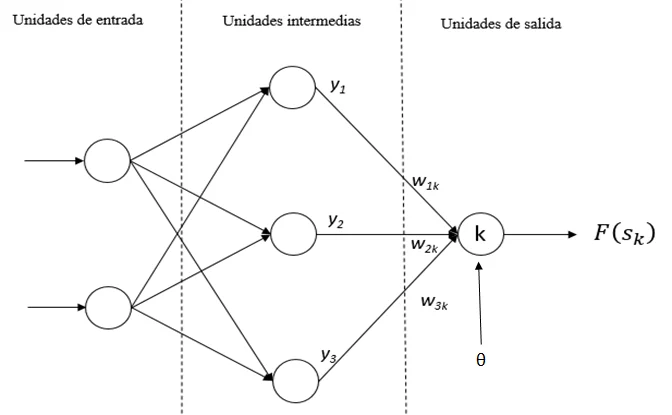
\includegraphics[width=0.7\linewidth]{figures/Simple_Neural_network.png}
    \caption{Esquema de una red neuronal simple. \citebox{firefly_ann_pretraining_researchgate_2026}}
    \label{fig: neural_network}
\end{figure}

Las funciones de activación más utilizadas en la práctica incluyen la sigmoide $\sigma(z) = 1/(1+e^{-z})$, la tangente hiperbólica $\sigma(z) = \tanh(z)$, y la unidad lineal rectificada (ReLU) $\sigma(z) = \max(0, z)$. La elección de la función de activación tiene consecuencias importantes sobre la dinámica del entrenamiento. Funciones como la sigmoide pueden producir gradientes que se desvanecen en redes profundas, mientras que la ReLU mitiga parcialmente este problema \citebox{schmidhuber2015deep}.

Una capa completa de la red consiste en $m$ neuronas que operan en paralelo sobre la misma entrada, produciendo un vector de salida $\mathbf{y} \in \mathbb{R}^m$:

\begin{equation} \label{eq: capa}
    \mathbf{y} = \sigma(\mathbf{W}\mathbf{x} + \mathbf{b})
\end{equation}

donde $\mathbf{W} \in \mathbb{R}^{m \times n}$ es la matriz de pesos de la capa y $\mathbf{b} \in \mathbb{R}^m$ el vector de sesgos.

Llegamos a la definición de \textit{deep learning}, que no es más que el uso de una red neuronal con muchas capas intermedias, lo que se conoce como red profunda. La expresión matemática que define una red profunda es una extensión de la\eqrefbox{eq: capa} pero para $L$ capas:

\begin{equation} \label{eq: red_profunda}
    f(\mathbf{x}) = \sigma_L(\mathbf{W}_L \cdots \sigma_2(\mathbf{W}_2 \, \sigma_1(\mathbf{W}_1 \mathbf{x} + \mathbf{b}_1) + \mathbf{b}_2) \cdots + \mathbf{b}_L)
\end{equation}

Los parámetros entrenables del modelo son el conjunto $\{\mathbf{W}_1, \mathbf{b}_1, \mathbf{W}_2, \mathbf{b}_2, \ldots, \mathbf{W}_L, \mathbf{b}_L\}$, cuyo número total crece con la anchura y la profundidad de la red.

El entrenamiento de una red neuronal se formula como un problema de optimización. Dado un conjunto de entrenamiento $\{(\mathbf{x}_n, y_n)\}_{n=1}^{N_T}$, se define una \textit{función de coste} (o función de pérdida) $C$ que mide la discrepancia entre las predicciones del modelo $f(\mathbf{x}_n)$ y las etiquetas verdaderas $y_n$. El objetivo es encontrar los parámetros $\boldsymbol{\theta} = \{\mathbf{W}_l, \mathbf{b}_l\}$ que minimizan $C$:

\begin{equation} \label{eq: optimizacion}
    \boldsymbol{\theta}^* = \arg\min_{\boldsymbol{\theta}} \; C(\boldsymbol{\theta}) = \arg\min_{\boldsymbol{\theta}} \; \frac{1}{N_T} \sum_{n=1}^{N_T} \mathcal{L}(f(\mathbf{x}_n; \boldsymbol{\theta}), y_n)
\end{equation}

donde $\mathcal{L}$ es una función de pérdida por muestra (por ejemplo, el error cuadrático medio o la entropía cruzada). Este es un problema de minimización en un espacio de alta dimensión, que se resuelve mediante variantes del \textit{descenso de gradiente} \citebox{schmidhuber2015deep}.

El algoritmo fundamental para calcular los gradientes necesarios es la \textit{backpropagation}, que aplica sistemáticamente la regla de la cadena del cálculo diferencial para propagar el error desde la capa de salida hacia las capas inferiores. Para un parámetro $\theta$ cualquiera de la red, el gradiente se calcula como:

\begin{equation} \label{eq: backprop}
    \frac{\partial C}{\partial \theta} = \frac{\partial C}{\partial \mathbf{y}_L} \cdot \frac{\partial \mathbf{y}_L}{\partial \mathbf{y}_{L-1}} \cdots \frac{\partial \mathbf{y}_{l+1}}{\partial \mathbf{y}_l} \cdot \frac{\partial \mathbf{y}_l}{\partial \theta}
\end{equation}

donde $\mathbf{y}_l$ es la salida de la capa $l$-ésima y cada factor $\partial \mathbf{y}_{l+1} / \partial \mathbf{y}_l$ es una matriz jacobiana, por lo que el orden de los productos es relevante. La actualización de los parámetros sigue entonces la regla $\theta \leftarrow \theta - \eta \, \partial C / \partial \theta$, donde $\eta > 0$ es la tasa de aprendizaje.

La diferencia fundamental entre las redes clásicas y las redes \textit{deep} radica en su capacidad de representación. Una red con una única capa oculta puede, en teoría, aproximar cualquier función continua con la suficiente anchura, pero resulta ineficiente para capturar estructuras jerárquicas, como las que están presentes en las imágenes o en el lenguaje natural \citebox{cybenko1989approximation, hornik1991approximation, cichocki2016tensor}. Las redes profundas, en cambio, aprenden representaciones en múltiples niveles de abstracción. Las capas más bajas detectan características primitivas como bordes o frecuencias, mientras que las superiores combinan estas primitivas para reconocer objetos complejos o conceptos semánticos \citebox{wang2023tensor}.

En clasificación de imágenes, las redes convolucionales han sido especialmente relevantes porque incorporan localidad espacial y pesos compartidos. Estas dos propiedades son adecuadas para datos visuales, porque los píxeles vecinos tienden a estar relacionados, y los mismos patrones pueden aparecer en distintas regiones de la imagen. La \figref{fig: 1} muestra algunas topologías básicas de redes neuronales.

\begin{figure}[H]
    \centering
    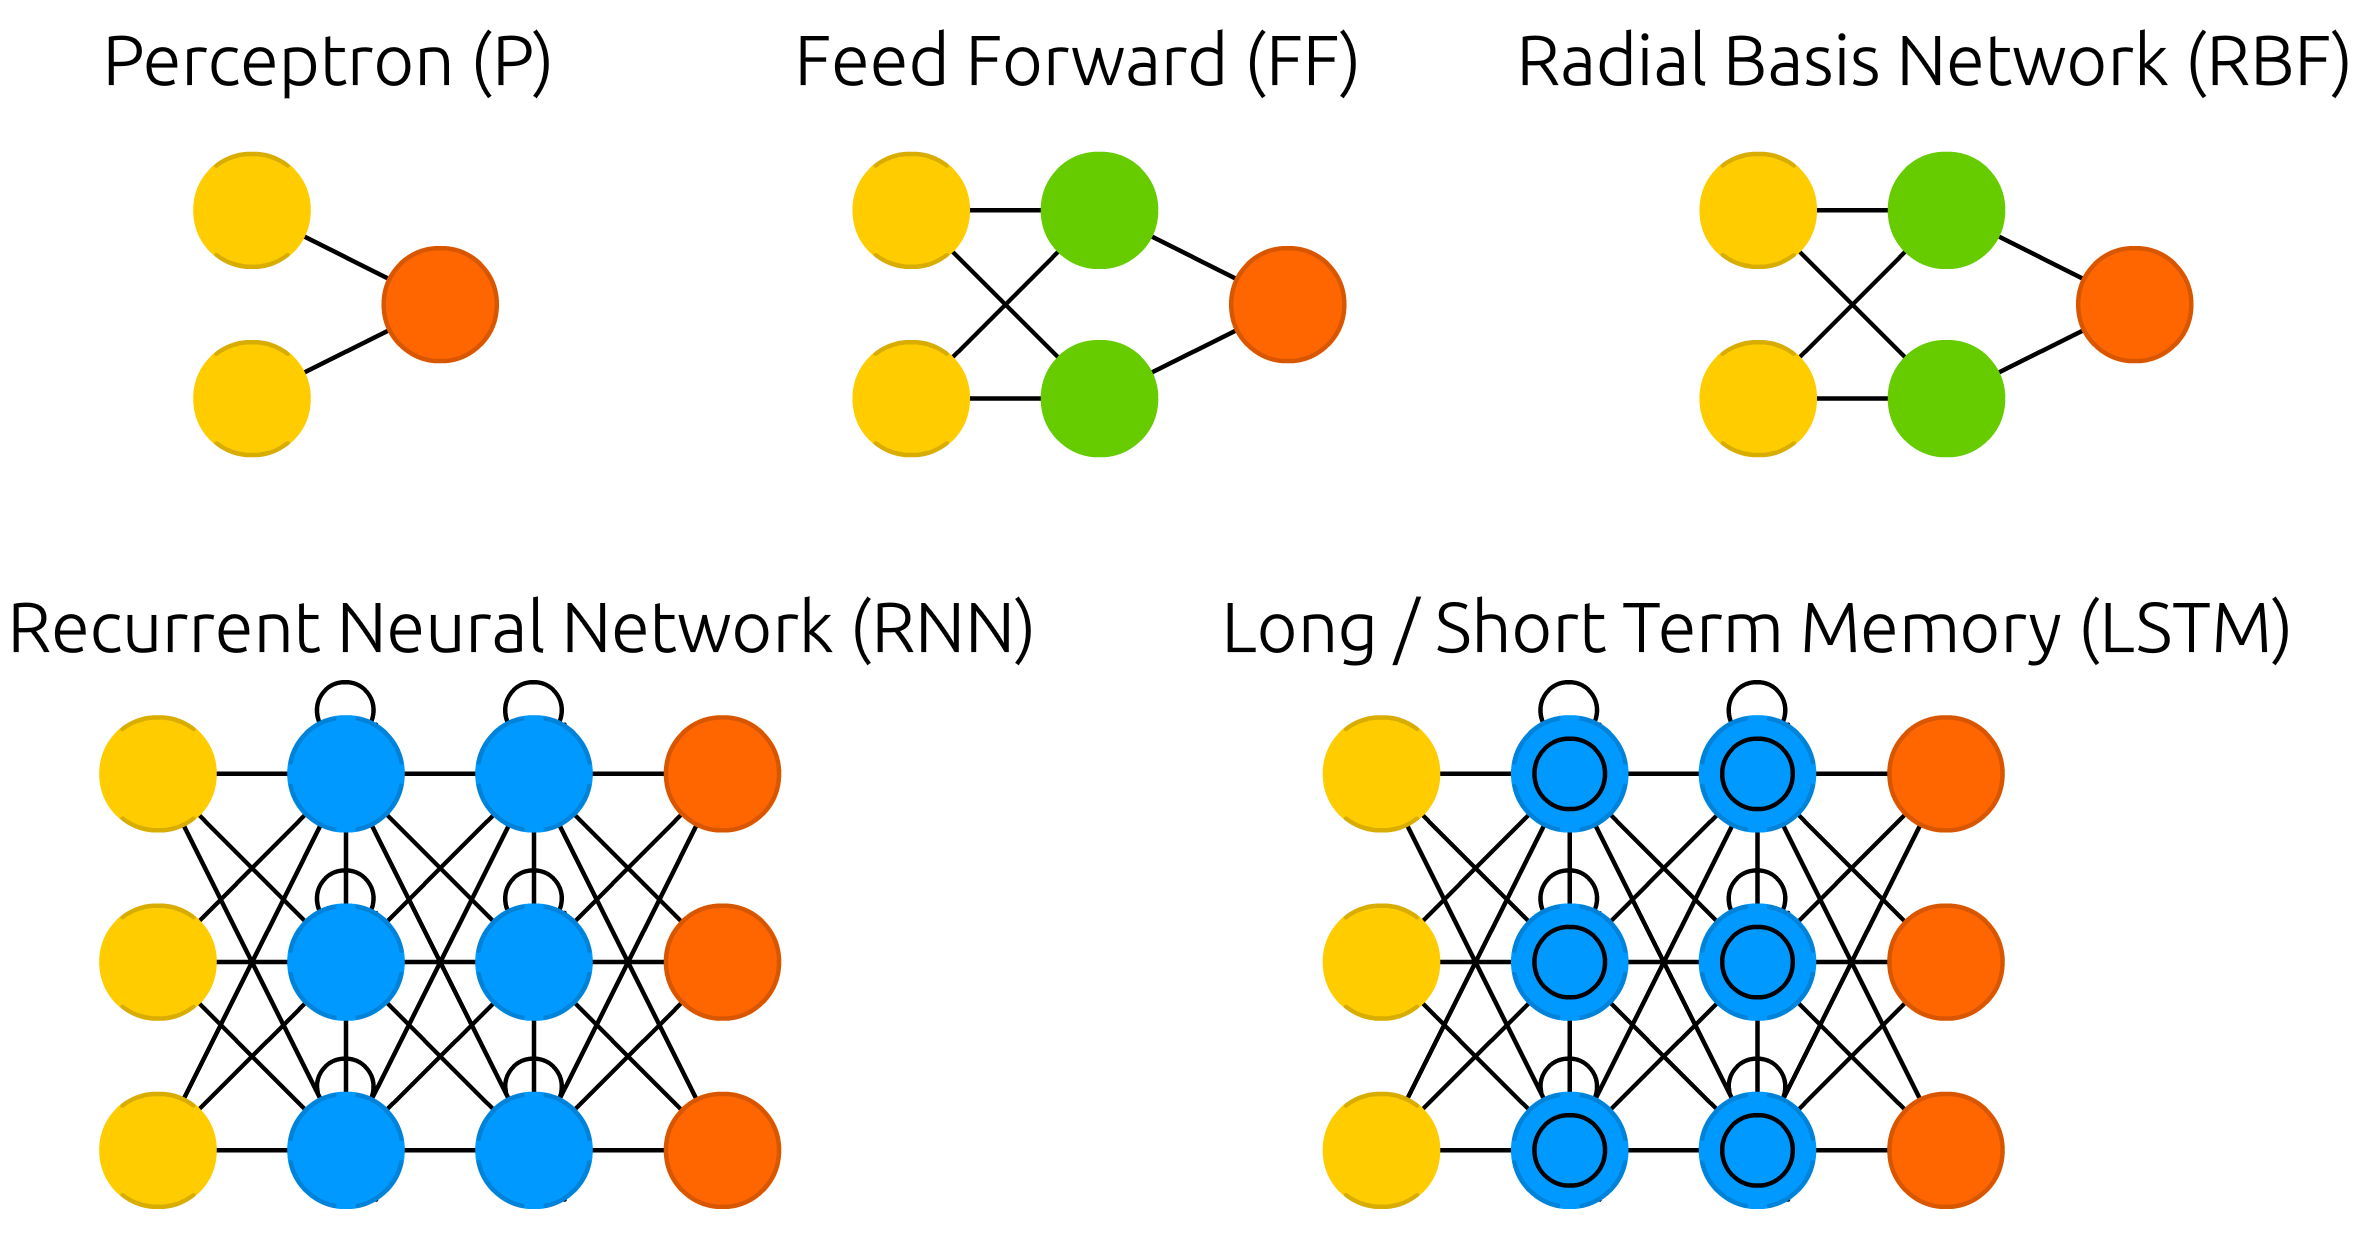
\includegraphics[width=0.78\linewidth]{figures/NeuralNetworks_recortada.png}
    \caption{Esquema de topologías básicas de redes neuronales, desde el perceptrón hasta arquitecturas con capas ocultas y conexiones recurrentes \citebox{vanveen2019zoo}.}
    \label{fig: 1}
\end{figure}

El éxito de estas arquitecturas no elimina sus limitaciones. Muchos modelos modernos alcanzan buenos resultados con un número elevado de parámetros y con un coste computacional considerable. Este TFG se sitúa en ese punto. Estudia si las TN pueden proporcionar modelos de clasificación estructurados, capaces de representar funciones complejas mediante factorizaciones tensoriales controladas.

\section{Tensores}

Antes de profundizar en el mundo de las TN es conveniente sentar primero las bases. Lo primero es entender qué es un tensor. Un tensor lo podemos ver definido de diferentes formas dependiendo del campo en el que estemos trabajando.

Desde un punto de vista computacional, los tensores son \textit{arrays} multidimensionales que generalizan de forma natural los conceptos de escalar, vector y matriz a dimensiones arbitrariamente superiores. Desde un punto de vista físico-matemático, los tensores son objetos matemáticos de orden superior, que representan relaciones multidimensionales entre distintas variables o grados de libertad. Dicho de otra forma, un tensor de orden $N$ es un objeto cuyos elementos tienen $N$ índices y están asociados a $N$ vectores base. \[R^{I_1 \times I_2 \times \cdots \times I_N}\] donde $N$ es el número de modos y las longitudes $I_1, \ldots, I_N$ representan las dimensiones de cada modo. \citebox{wang2023tensor}

Bajo esta definición, los escalares son tensores de orden cero, los vectores son tensores de orden 1, y las matrices son tensores de orden 2; todo caso superior constituye propiamente lo que en la literatura se denomina, tensor de alto orden. En la notación convencional, se distinguen los diferentes objetos según su orden: las letras minúsculas en cursiva ($a$) denotan escalares, las letras minúsculas en negrita ($\mathbf{a}$) denotan vectores, las letras mayúsculas en negrita ($\mathbf{A}$) denotan matrices, y las letras mayúsculas en tipografía cursiva en negrita ($\boldsymbol{\mathcal{A}}$) denotan tensores de orden superior. \citebox{wang2023tensor}

La intuición física detrás de los tensores resulta natural cuando se considera que muchos fenómenos del mundo real son inherentemente multidimensionales. Una imagen en color, por ejemplo, es un tensor de orden tres: altura, anchura y canales cromáticos. Los datos de resonancia magnética funcional (fMRI) constituyen tensores de orden cuatro. En mecánica cuántica, las funciones de onda de sistemas de muchos cuerpos son, igualmente, tensores de alto orden \citebox{wang2023tensor}.

El concepto de tensor tiene raíces en el siglo XIX, ligado al desarrollo del cálculo diferencial absoluto por Ricci-Curbastro y Levi-Civita, aunque fue la formulación de la relatividad general por Einstein en 1915 la que consagró los tensores como herramienta fundamental de la física matemática. La descripción matemática de un tensor es la siguiente:
\begin{equation} \label{eq: 1}
    \boldsymbol{\mathcal{T}} = \sum_{i_1, i_2,..., i_n} \tensor{T}{_{i_1}_{i_2}_{...}_{i_n}} \hat{b}_{i_1} \hat{b}_{i_2}...\hat{b}_{i_n}
\end{equation}

La operación central en el álgebra tensorial es la contracción tensorial. Dados dos tensores $\boldsymbol{\mathcal{T}}$ y $\boldsymbol{\mathcal{R}}$, de orden $n$ y $m$ respectivamente, con elementos $\tensor{T}{_{i_1}_{i_2}_{...}_{i_n}}$ y $\tensor{R}{_{j_1}_{j_2}_{...}_{j_m}}$ y en la misma base ortonormal $\hat{b}_{i}$, diremos que el tensor $\boldsymbol{\mathcal{C}}$ es la contracción de ambos tensores por sus últimos $q$ índices cuando:

\begin{equation} \label{eq: 2}
    \mathcal{C} = \sum_{i_1, i_2,...,i_{n-q},j_1,j_2,...,j_{m-q}} \tensor{C}{_{i_1}_{i_2}_{...}_{i_{n-q}}_{,}_{j_1}_{j_2}_{...}_{j_{m-q}}} \hat{b}_{i_1}\hat{b}_{i_2}...\hat{b}_{n-q}\hat{b}_{j_1}\hat{b}_{j_2}...\hat{b}_{m-q}
\end{equation}

siendo sus elementos

\begin{equation} \label{eq: 3}
    \tensor{C}{_{i_1}_{i_2}_{...}_{i_{n-q}}_{,}_{j_1}_{j_2}_{...}_{j_{m-q}}} = \sum_{k_1, k_2,...,k_{q}} \tensor{T}{_{i_1}_{i_2}_{...}_{i_{n-q}}_{,}_{k_1}_{k_2}_{...}_{k_{q}}} \tensor{R}{_{j_1}_{j_2}_{...}_{j_{m-q}}_{,}_{k_1}_{k_2}_{...}_{k_{q}}}
\end{equation}

De esta definición podemos sacar que la contracción tensorial es la operación mediante la cual dos tensores se contraen en un único tensor a lo largo de sus pares de índices asociados. Existen formas diferentes de contracciones, algunas implican más de dos tensores o un índice repetido en más de dos tensores o incluso repetidos en el mismo tensor. El caso más familiar de contracción tensorial es la multiplicación matricial: \[\mathbf{AB} = \sum_{k} A_{ik}B_{kj}\hat{b}_i\hat{b}_j\] o el producto escalar entre dos vectores: \[\mathbf{v}\cdot\mathbf{w} = \sum_i v_iw_i\]

Entre las operaciones tensoriales fundamentales cabe destacar la traza de una matriz:

\begin{equation}
    Tr(\mathbf{A}) = \sum_{i}A_{ii}
\end{equation}

Esto sería la contracción de una matriz consigo misma a través de sus índices repetidos. Debido a esta operación podemos ver que, un tensor también sirve como mapeo entre dos espacios vectoriales. Esto es un tensor, que recibe otro tensor y devuelve un tercer tensor. Por cada par de índices contraído estamos mezclando componentes de los tensores de entrada, reduciendo en 2 el orden total. Los índices que no han sido contraídos, en cambio, no desaparecen, sino que sobreviven como índices libres del tensor de salida. Así, al contraer un tensor de orden $n$ con uno de orden $m$ a lo largo de $q$ pares de índices, el tensor resultante tiene orden $n + m - 2q$, en consonancia con la \eqrefbox{eq: 3}.

\section{Notación diagramática de Penrose y definición de Tensor Network}

La representación algebraica de las contracciones tensoriales, aunque precisa, se vuelve rápidamente inmanejable a medida que aumenta el número de tensores y la complejidad de sus conexiones. Fue Roger Penrose \citebox{penrose1971applications} quien, a principios de la década de 1970, introdujo la notación diagramática para tensores, proporcionando una alternativa visual que transformó la manera en que se razona sobre estas estructuras. Los diagramas de redes tensoriales se utilizan hoy en día, en investigación, para describir algoritmos cuánticos y algoritmos de \textit{machine learning} \citebox{wang2023tensor}.

La idea central de la notación de Penrose es representar cada tensor como un nodo del que emanan tantas aristas como índices tenga el tensor. Concretamente, un nodo con una sola arista representa un vector $\mathbf{a} \in \mathbb{R}^I$; un nodo con dos aristas representa una matriz $\mathbf{A} \in \mathbb{R}^{I \times J}$; y un nodo con tres aristas representa un tensor $\boldsymbol{\mathcal{A}} \in \mathbb{R}^{I_1 \times I_2 \times I_3}$. Para indicar que un par de índices tensoriales está siendo contraído, ambas aristas se unen mediante una línea. Por ejemplo, la contracción de un tensor de orden uno con uno de orden dos es la multiplicación matriz-vector habitual. Las aristas que no se conectan a ningún otro tensor se denominan aristas libres, y el número de estas aristas en el diagrama resultante es precisamente el orden del tensor final. Dos nodos que no están unidos mediante aristas, representan el producto tensorial entre ellos.

\begin{figure}[H]
    \centering
    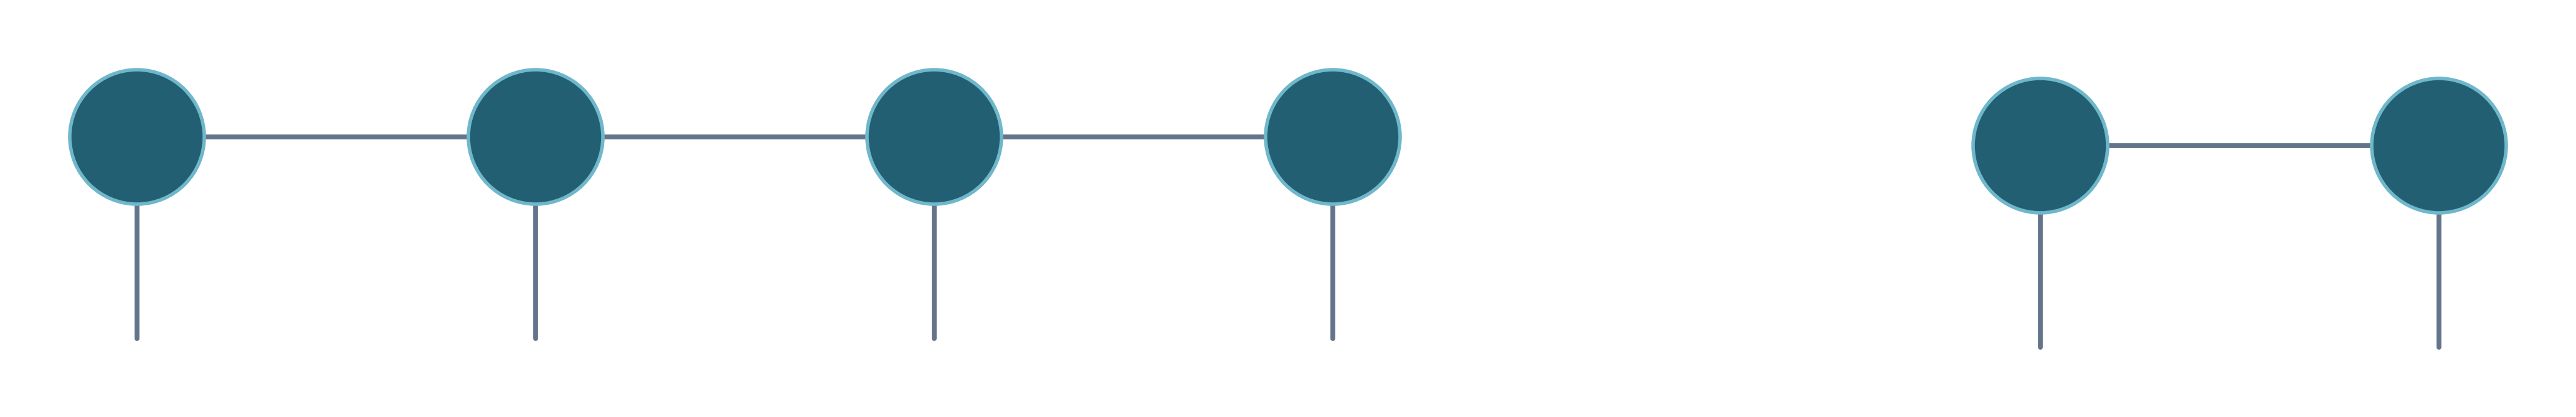
\includegraphics[width=1.0\linewidth]{figures/TN_invented.png}
    \caption{Representación de una TN inventada. En esta representación se pueden identificar muchas de las operaciones descritas en esta sección. Elaboración propia usando la librería Tensor-Network-Editor, creada por Alejandro Mata Ali. \citebox{Mata_Ali_Tensor_Network_Editor_2026}}
    \label{fig:Invented_TN}
\end{figure}

La notación gráfica tensorial ofrece numerosas ventajas sobre la notación tradicional. En forma gráfica, los índices no necesitan nombres ni etiquetas; operaciones como el producto escalar, la traza tensorial y la contracción pueden expresarse sin notación adicional; y el orden del tensor resultante puede leerse simplemente contando el número de aristas libres. En particular, si en el diagrama no quedan aristas libres tras todas las contracciones, el resultado es necesariamente un escalar. Esta propiedad convierte los diagramas en una herramienta de verificación inmediata de la consistencia dimensional de operaciones complejas \citebox{stoudenmire2017supervisedlearningquantuminspiredtensor}. Sobre esta base visual puede introducirse ya, de manera natural, el concepto de \textit{Tensor Network (TN)}.

Una TN es, en esencia, una representación gráfica de una ecuación multilineal entre diferentes tensores. Esta representación se apoya en la notación diagramática de Penrose, que con el tiempo se ha ido adaptando a las necesidades de disciplinas como la física, las matemáticas o la ciencia computacional \citebox{biamonte2017tensornetworksnutshell}. Puede verse un ejemplo en la \figref{fig: TensorNetwork}, donde aparece la TN que representa el 2-tensor $\tensor{T}{_{i}_{p}}$ cuyos elementos se obtienen mediante la operación de contracción

\begin{equation} \label{eq: 5}
\tensor{T}{_{i}_{p}} = \sum_{j, k, l, m, n, o}\tensor{A}{_{i}_{j}_{k}_{l}} \tensor{B}{_{j}_{m}}\tensor{C}{_{k}_{m}_{n}}\tensor{D}{_{l}_{o}}\tensor{E}{_{n}_{o}_{p}}
\end{equation}

\begin{figure}[H]
\centering
\makebox[\textwidth]{%
  \begin{minipage}{1.1\textwidth}
    \centering
    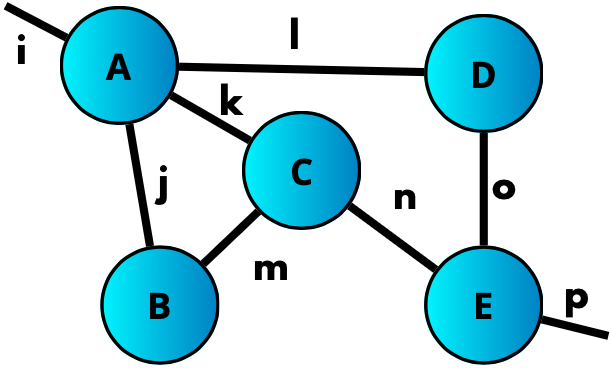
\includegraphics[scale=0.45]{figures/TensorNetwork_example.png}
    \caption{Ejemplo de representación diagramática para un tensor. Fuente:\citebox{2024arXiv240411277M}}
    \label{fig: TensorNetwork}
  \end{minipage}%
}
\end{figure}

Desde un punto de vista computacional, una Tensor Network no debe entenderse únicamente como un dibujo, sino como una forma factorizada de representar un tensor de alto orden. En lugar de almacenar explícitamente todos los elementos del tensor completo, se almacena una colección de tensores de menor orden, conectados entre sí mediante índices compartidos. Cada tensor de la red suele denominarse también núcleo, bloque o tensor local, dependiendo del contexto \citebox{wang2023tensor}.

En una red tensorial aparecen dos tipos de índices con papeles distintos. Los índices que quedan libres tras realizar las contracciones corresponden a los índices del tensor final representado por la red. En problemas de física cuántica suelen denominarse índices físicos, mientras que en aplicaciones de aprendizaje automático pueden interpretarse como posiciones de entrada, características o salidas del modelo. Por otro lado, los índices que conectan dos tensores internos se denominan índices virtuales o índices de enlace. Estos índices no aparecen en el tensor final, ya que se suman durante la contracción, pero controlan cuánta información puede transmitirse entre distintas partes de la red.

La dimensión de estos índices internos, denominada dimensión de enlace, es uno de los parámetros más importantes de una Tensor Network. Si la dimensión de enlace es pequeña, la red contiene pocos parámetros y la representación es muy compacta, pero también queda limitada su capacidad para representar correlaciones complejas. Si la dimensión de enlace aumenta, la red gana expresividad, aunque también crecen el número de parámetros y el coste computacional de las contracciones. Por tanto, la dimensión de enlace desempeña un papel análogo al de un hiperparámetro que regula el compromiso entre compacidad y capacidad de representación.

La operación fundamental en una Tensor Network es la contracción. Contraer una red significa sumar sobre todos los índices internos compartidos hasta obtener el tensor final, que queda determinado únicamente por sus índices libres. Aunque algebraicamente esta operación puede escribirse como una suma sobre muchos índices, la notación diagramática permite visualizarla de forma más intuitiva; las aristas conectadas se eliminan al contraerse, mientras que las aristas libres permanecen como índices del resultado. Además, el orden en el que se realizan las contracciones puede afectar de forma significativa al coste computacional, por lo que una misma red puede ser más o menos eficiente dependiendo de la estrategia de contracción empleada \citebox{wang2023tensor}.

\section{Tensor Networks y reducción de dimensionalidad}

La motivación fundamental para el uso de las Tensor Networks es de naturaleza computacional. Un tensor de orden $N$ cuyos índices toman cada uno $d$ valores posee $d^N$ componentes, un número que crece exponencialmente con el orden del tensor y que hace inviable su almacenamiento y manipulación directos incluso para valores moderados de $N$ y $d$. Este fenómeno se conoce como \textit{maldición de la dimensionalidad} \citebox{wang2023tensor}.

El mismo problema aparece de forma natural en la física cuántica de muchos cuerpos, que es precisamente el contexto en el que surgieron las TN. Un estado cuántico general de $N$ subsistemas con dimensión local $d$ se escribe como

\begin{equation} \label{eq: estado_general}
    \ket{\psi} =
    \sum_{s_1,\ldots,s_N}
    C_{s_1\ldots s_N}\,
    \ket{s_1}\otimes\cdots\otimes\ket{s_N},
\end{equation}

donde el tensor de coeficientes $C_{s_1\ldots s_N}$ tiene de nuevo $d^N$ componentes. Sin embargo, los estados físicamente relevantes rara vez ocupan todo ese espacio con la máxima complejidad posible, porque sus correlaciones y su entrelazamiento suelen estar limitados, lo que permite representarlos de forma mucho más compacta de lo que sugiere el conteo $d^N$ \citebox{schollwock2011dmrg}.

La idea central de las Tensor Networks consiste en aprovechar esa estructura. En lugar de almacenar explícitamente el tensor completo, se representa como el resultado de contraer un conjunto de tensores de menor orden conectados entre sí mediante índices de enlace. Si las dimensiones de esos índices internos se mantienen acotadas, el número total de parámetros crece de forma polinómica e incluso lineal en algunas topologías, en lugar de exponencial con el número de modos \citebox{wang2023tensor, stoudenmire2017supervisedlearningquantuminspiredtensor}.

Esta reducción no es gratuita. Al fijar una topología concreta y unas dimensiones de enlace finitas se restringe la familia de tensores que pueden representarse de forma eficiente. Por ello, una Tensor Network debe entenderse como una aproximación estructurada; solo resulta eficaz cuando la estructura de correlaciones del problema es compatible con la topología elegida. Esta distinción es especialmente importante en \textit{machine learning}, donde la red tensorial no se limita a comprimir un tensor ya conocido, sino que se utiliza como una arquitectura entrenable cuyos parámetros se ajustan a partir de los datos.

Esta observación se traslada al \textit{machine learning} mediante una analogía útil. Un modelo de clasificación no necesita representar una función arbitraria sobre todas las entradas posibles, sino una función que aproveche las regularidades de los datos. Las Tensor Networks imponen una estructura de bajo rango o de conectividad concreta sobre el tensor de pesos, de modo que el número de parámetros permanece controlado siempre que las dimensiones internas, llamadas dimensiones de enlace, se mantengan acotadas \citebox{cichocki2016tensor, wang2023tensor}.

\section{Descomposiciones tensoriales fundamentales}

Para comprender cómo se construyen las representaciones mediante TN, conviene introducir primero algunas descomposiciones tensoriales básicas. Cada una puede entenderse como una forma distinta de imponer estructura sobre un tensor de alto orden. La descomposición CP lo expresa como una suma de términos separables; la de Tucker introduce un núcleo central que acopla varios factores; y el formato Tensor Train (TT), conocido en física como Matrix Product State (MPS), organiza la información en una cadena de tensores conectados por índices de enlace. Cada uno ofrece un compromiso diferente entre compacidad, expresividad y coste computacional, como se verá a lo largo de la sección.

La herramienta algebraica fundamental es la descomposición en valores singulares (SVD). Dada una matriz $\mathbf{A} \in \mathbb{R}^{M \times N}$, la SVD la factoriza como

\begin{equation} \label{eq: svd}
    \mathbf{A} = \mathbf{U} \boldsymbol{\Sigma} \mathbf{V}^\top ,
\end{equation}

donde $\mathbf{U}$ y $\mathbf{V}$ son matrices ortogonales, y $\boldsymbol{\Sigma}$ contiene los valores singulares $\sigma_1 \geq \sigma_2 \geq \cdots \geq 0$. La importancia de la SVD en TN se debe a que permite obtener la mejor aproximación de bajo rango en norma de Frobenius. Al conservar solo los $R$ valores singulares dominantes se obtiene la matriz de rango $R$ que minimiza el error de reconstrucción, resultado conocido como teorema de Eckart--Young \citebox{wang2023tensor}.

Una primera generalización del rango matricial a tensores de orden superior es la descomposición CP. Dado un tensor $\boldsymbol{\mathcal{X}} \in \mathbb{R}^{I_1 \times \cdots \times I_N}$, CP lo aproxima como suma de $R$ tensores de rango 1:

\begin{equation} \label{eq: CP}
    \boldsymbol{\mathcal{X}} \approx \sum_{r=1}^{R} 
    \mathbf{a}_r^{(1)} \circ \mathbf{a}_r^{(2)} \circ \cdots \circ \mathbf{a}_r^{(N)} ,
\end{equation}

donde $\circ$ denota el producto exterior y $R$ es el rango CP. Esta representación es muy compacta, con $R \sum_{n=1}^{N} I_n$ parámetros, pero presenta dificultades prácticas; determinar el rango CP es un problema NP-difícil y los métodos de ajuste habituales no garantizan alcanzar el óptimo global \citebox{kolda2009tensor, wang2023tensor}. En notación diagramática, CP se representa mediante factores vectoriales conectados a un nodo central diagonal.

La descomposición de Tucker es más flexible. En lugar de una única suma de componentes de rango 1, introduce un tensor núcleo $\boldsymbol{\mathcal{G}}$ que modela las interacciones entre los factores:

\begin{equation} \label{eq: Tucker}
    \tensor{\mathcal{X}}{_{i_1}_{i_2}_{...}_{i_N}} \approx 
    \sum_{r_1=1}^{R_1} \cdots \sum_{r_N=1}^{R_N}
    \tensor{\mathcal{G}}{_{r_1}_{r_2}_{...}_{r_N}}
    \tensor{A}{^{(1)}_{i_1 r_1}}
    \tensor{A}{^{(2)}_{i_2 r_2}}
    \cdots
    \tensor{A}{^{(N)}_{i_N r_N}} .
\end{equation}

Los valores $R_1,\ldots,R_N$ son los rangos de Tucker y pueden ser distintos para cada modo. Si las matrices de factores son ortogonales, se obtiene la Higher-Order Singular Value Decomposition (HOSVD), una extensión natural de la SVD al caso tensorial \citebox{wang2023tensor}. CP puede verse como un caso particular de Tucker cuando el núcleo es superdiagonal y todos los rangos coinciden. Sin embargo, el núcleo de Tucker contiene $\prod_{n=1}^{N} R_n$ parámetros, por lo que el coste vuelve a crecer exponencialmente con el orden del tensor.

Esta limitación motiva formatos más escalables como Tensor Train (TT), conocido en física como Matrix Product State (MPS) \citebox{oseledets2011tt, schollwock2011dmrg}. TT representa un tensor de orden $N$ como una cadena de tensores locales $\boldsymbol{\mathcal{G}}^{(n)} \in \mathbb{R}^{R_{n-1} \times I_n \times R_n}$ conectados mediante índices virtuales. Su número de parámetros es

\[
    \sum_{n=1}^{N} R_{n-1} I_n R_n ,
\]

que crece linealmente con $N$ si los rangos se mantienen acotados. Además, la descomposición TT puede construirse mediante SVD sucesivas, lo que proporciona estabilidad numérica y permite controlar el error mediante el truncamiento de valores singulares \citebox{wang2023tensor, oseledets2011tt}. Desde la perspectiva cuántica, los rangos TT coinciden con los rangos de Schmidt de las biparticiones correspondientes, conectando esta construcción con la noción de entrelazamiento discutida anteriormente \citebox{schollwock2011dmrg}.

La \tabref{tab:comparativa_descomposiciones} resume las diferencias principales entre los formatos anteriores.

\begin{table}[H]
\centering
\renewcommand{\arraystretch}{1.3}

\begin{tabularx}{\textwidth}{|l|c|X|}
\hline
\textbf{Formato} & \textbf{Parámetros} & \textbf{Observaciones} \\
\hline
CP &
$R \sum_n I_n$ &
Muy compacta, pero el rango CP es difícil de determinar. \\
\hline
Tucker &
$\prod_n R_n + \sum_n I_n R_n$ &
Flexible, pero el núcleo crece exponencialmente con el orden. \\
\hline
TT/MPS &
$\sum_n R_{n-1} I_n R_n$ &
Escalado lineal para rangos fijos; construible mediante SVD sucesivas. \\
\hline
\end{tabularx}

\caption{Comparación entre las descomposiciones CP, Tucker y TT/MPS.}
\label{tab:comparativa_descomposiciones}
\end{table}

\begin{figure}[H]
    \centering
    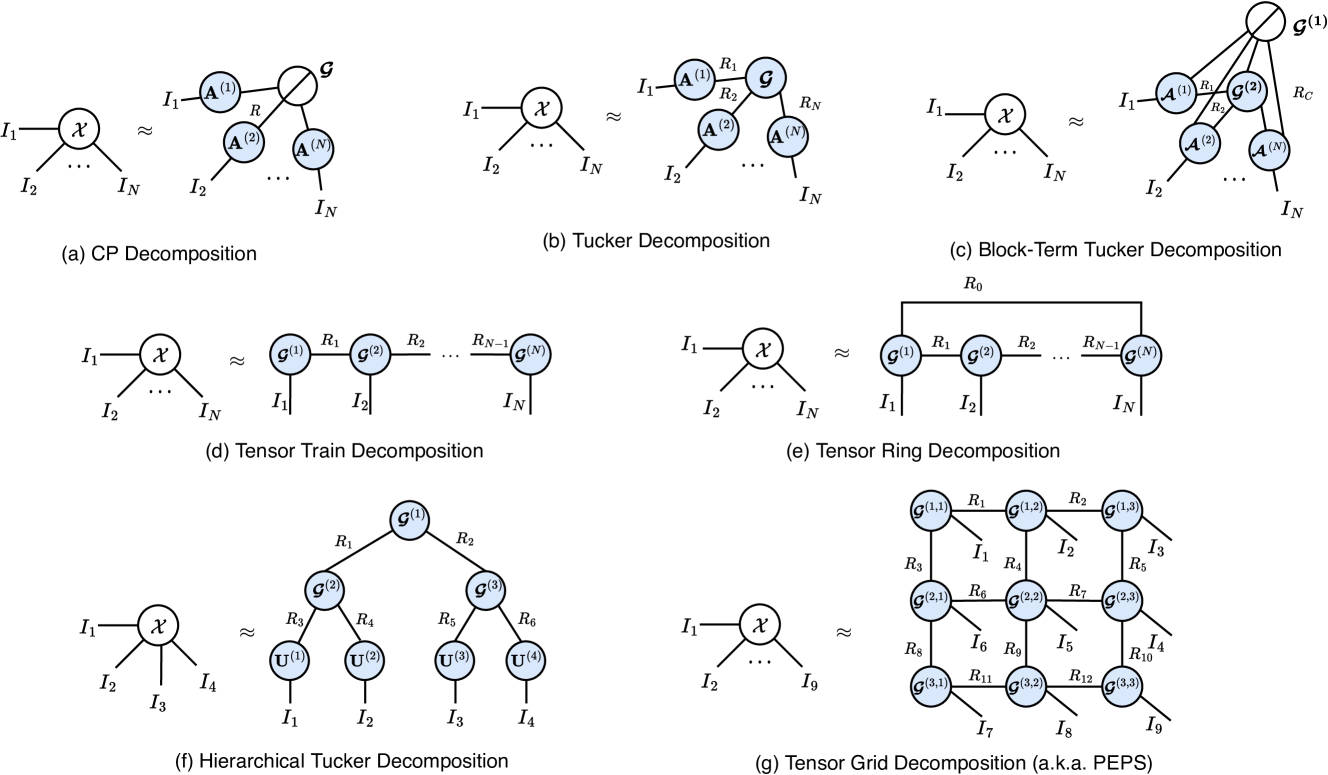
\includegraphics[width=0.9\linewidth]{figures/Decompositions_in_TN.png}
    \caption{Diagramas TN de algunas descomposiciones tensoriales populares. (a) El formato CP descompone un tensor \(X\) en una suma de varios tensores de rango 1 $a^{(1)}_{:,r} \circ a^{(2)}_{:,r} \circ \cdots \circ a^{(N)}_{:,r}.$ (b) La descomposición de Tucker descompone un tensor \(X\) en un tensor núcleo \(G\) multiplicado por una matriz \(A^{(n)}\) a lo largo del modo \(n\)-ésimo. (d) La descomposición TT descompone un tensor \(X\) en una multiplicación lineal de un conjunto de tensores núcleo de tercer orden $G^{(2)} \cdots G^{(N-1)}$ y dos matrices \(G^{(1)}\) y \(G^{(N)}\). (g) La descomposición en malla tensorial, también conocida como PEPS, representa un tensor de alta dimensión como una malla bidimensional de tensores interconectados de menor rango, donde cada nodo se conecta con sus vecinos para capturar eficientemente correlaciones espaciales en sistemas con interacciones locales. Los paneles (c), (e) y (f) corresponden, respectivamente, a las descomposiciones en términos de bloque, Tensor Ring (TR) y jerárquica de Tucker (HT), no empleadas en este trabajo. \citebox{wang2023tensor}}
    \label{fig: cp_decomposition}
\end{figure}

\section{Topologías principales de Tensor Networks}

La topología de una Tensor Network determina qué correlaciones puede representar de forma eficiente y con qué coste computacional. En esta sección se detallan las topologías de TN más utilizadas y más relevantes en la literatura.

\subsection{Matrix Product State / Tensor Train}

El \textit{Matrix Product State} (MPS), conocido en la literatura matemática como Tensor Train (TT), es la topología de TN más estudiada y mejor comprendida. Consiste en una cadena lineal de $N$ tensores conectados secuencialmente mediante índices virtuales de dimensión $D$. Los tensores de los extremos tienen dos índices y los intermedios tres, un índice asociado a la posición de entrada y dos índices de enlace que conectan con los vecinos. Ambos nombres describen la misma topología y la diferencia está en el contexto de uso. En física la MPS se introdujo para representar estados cuánticos de muchos cuerpos, mientras que en análisis numérico y aprendizaje automático el formato TT se emplea como herramienta de compresión y parametrización eficiente de tensores de alta dimensión \citebox{oseledets2011tt}.

Los índices internos de la cadena reciben el nombre de rangos TT o dimensiones de enlace, y determinan cuánta información puede transmitirse entre las distintas partes de la cadena. Dimensiones pequeñas dan un modelo muy compacto pero con capacidad limitada para representar correlaciones entre posiciones alejadas; al aumentarlas, la representación gana expresividad a costa de más parámetros y contracciones más costosas. En aplicaciones de aprendizaje automático, la dimensión de enlace actúa por tanto como un hiperparámetro que regula la complejidad del modelo \citebox{stoudenmire2017supervisedlearningquantuminspiredtensor}.

Una ventaja relevante del formato TT es que puede construirse aplicando descomposiciones en valores singulares de forma sucesiva a distintas matricizaciones del tensor. Este procedimiento, conocido como TT-SVD, proporciona una forma numéricamente estable de obtener una aproximación con rangos controlados \citebox{oseledets2011tt}, y conecta la MPS con la SVD introducida anteriormente: no es solo una arquitectura inspirada en la física, sino también una herramienta de reducción de dimensionalidad.

Desde el punto de vista físico, la MPS es la representación más natural de los estados fundamentales de los sistemas cuánticos unidimensionales con interacciones locales, lo que explica su relevancia en este campo. Una propiedad característica es que las correlaciones que puede representar decaen exponencialmente con la distancia entre posiciones: la función de correlación entre las posiciones $i$ y $j$ satisface:

\begin{equation}
  \langle O_i O_j \rangle - \langle O_i \rangle \langle O_j \rangle \sim e^{-|i-j|/\xi}   
\end{equation}

donde $\xi$ es una longitud de correlación que depende de la dimensión de enlace $D$ \citebox{stoudenmire2017supervisedlearningquantuminspiredtensor}. Por ello la MPS captura con eficiencia las correlaciones de corto alcance, pero puede requerir dimensiones de enlace elevadas para las de largo alcance.

No obstante, la MPS organiza la información en una cadena. Esto es natural para datos secuenciales, pero menos adecuado para imágenes, que poseen una estructura espacial bidimensional. Aplicar una MPS a una imagen obliga a ordenar sus posiciones de entrada en una secuencia. Esa ordenación puede conservar parcialmente la vecindad espacial, por ejemplo mediante un recorrido en zigzag, pero transforma inevitablemente una geometría bidimensional en una unidimensional. Esta limitación es una de las motivaciones para considerar topologías jerárquicas, como las Tree Tensor Networks, en problemas de visión artificial.

Una forma especialmente interesante de utilizar una MPS en aprendizaje supervisado consiste en emplearla como parametrización del tensor de pesos de un clasificador. En un modelo lineal convencional, la entrada se representa mediante un vector de características que se multiplica por una matriz de pesos. En el enfoque tensorial, la entrada se transforma primero en un tensor de alto orden mediante un mapa local de características y el tensor de pesos se representa de forma comprimida mediante una MPS \citebox{stoudenmire2017supervisedlearningquantuminspiredtensor}. De manera esquemática, si una entrada $x$ se descompone en varias posiciones $x_1,\ldots,x_N$, a cada una se le aplica un mapa local

\[ \phi(x_j) \in \mathbb{R}^{d}, \]

con $d$ la dimensión local, y la representación completa de la entrada se obtiene como producto tensorial de todos los vectores locales:

\[ \Phi(x)=\phi(x_1)\otimes \phi(x_2)\otimes \cdots \otimes \phi(x_N). \]

Aunque formalmente $\Phi(x)$ pertenece a un espacio de dimensión $d^N$, no es necesario construirlo de forma explícita, porque la estructura de la red permite trabajar con esta representación de manera implícita mediante contracciones sucesivas. Para clasificación multiclase se introduce un índice adicional asociado a la etiqueta de clase, de modo que la MPS representa un tensor de pesos $W^{\ell}$ y, al contraerlo con la representación de entrada, se obtiene una puntuación por clase:

\[ f^{\ell}(x)= W^{\ell}\cdot \Phi(x). \]

La clase predicha es la de mayor puntuación. En el lenguaje habitual del \textit{deep learning}, estas puntuaciones se interpretan como los valores previos a la normalización probabilística final del clasificador. Así, la MPS no se limita a comprimir un tensor ya conocido, sino que define directamente la forma de los parámetros que se optimizan, y su dimensión de enlace controla la complejidad del clasificador.

Este esquema fue explorado por Stoudenmire y Schwab, que aplicaron una MPS a la clasificación de dígitos manuscritos sobre MNIST, ordenando los píxeles en una secuencia mediante un recorrido en zigzag para preservar en parte la proximidad espacial, y alcanzaron un error de test inferior al $1\%$ \citebox{stoudenmire2017supervisedlearningquantuminspiredtensor}. Este resultado ilustra el potencial de la MPS como clasificador entrenable, pero también se hace evidente la necesidad de linealizar una imagen bidimensional antes de introducirla en la red, que es su gran limitación.

\subsection{Tree Tensor Network}

Una \textit{Tree Tensor Network} (TTN) organiza los tensores siguiendo una estructura jerárquica en forma de árbol. En lugar de propagar la información a lo largo de una cadena, asocia los tensores de la capa más baja (las \textit{hojas} o \textit{leaves} en inglés) a las posiciones de entrada y los contrae por grupos hacia tensores de capas superiores, reduciendo progresivamente el número de índices hasta llegar a un único tensor raíz que produce la salida. Los tensores de los niveles inferiores combinan información local, mientras que los superiores integran representaciones cada vez más globales, de modo que la red construye una jerarquía de características sobre la que se realiza la clasificación.

La diferencia esencial con una MPS es la forma en que se propagan las dependencias entre posiciones de entrada. En una cadena, dos posiciones alejadas solo se comunican a través de todos los tensores intermedios; en un árbol, en cambio, basta ascender unos pocos niveles hasta un nodo común, de manera que la distancia efectiva entre dos hojas crece como $\mathcal{O}(\log N)$ en lugar de linealmente \citebox{wang2023tensor, evenbly2011tensor}. Esta geometría hace que la TTN sea más eficiente que la MPS para combinar información lejana y, por tanto, para capturar correlaciones de largo alcance.

Al igual que en una MPS, la dimensión de los índices internos regula el compromiso entre compacidad y expresividad. Si es demasiado pequeña, la red pierde información relevante durante la compresión jerárquica; si es demasiado grande, gana capacidad pero aumentan el número de parámetros y el coste de entrenamiento. Existe, además, una decisión estructural que no es neutra: la forma concreta del árbol fija de antemano qué grupos de entradas se combinan primero y cuáles solo se encuentran en niveles superiores, lo que condiciona el tipo de dependencias que el modelo representa con mayor facilidad. En problemas de imágenes esta cuestión es especialmente relevante, ya que la organización espacial de la entrada influye en qué regiones conviene agrupar antes.

En física, la TTN se emplea para representar estados con una estructura de entrelazamiento jerárquica, como la que aparece en ciertos sistemas con simetría de escala. En \textit{machine learning}, su organización en árbol resulta natural para datos con estructura jerárquica intrínseca \citebox{wang2023tensor}. Esta correspondencia es la que motiva su uso en este trabajo. Aunque una TTN no reproduce de forma exacta la geometría bidimensional de una imagen, sí ofrece un mecanismo para agrupar posiciones de entrada y combinar la información de manera progresiva. Por ello la TTN no se aplica aquí directamente sobre los píxeles, sino sobre una secuencia de vectores de características obtenida tras una etapa inicial de extracción visual, un planteamiento híbrido que se detalla en la metodología.

La estructura de árbol también introduce una limitación. Al no contener ciclos, la información entre dos ramas distintas solo puede propagarse a través de su nodo ancestro común, lo que restringe la capacidad de la red para capturar correlaciones entre nodos situados en ramas separadas. Esta restricción es la que motivó el desarrollo de arquitecturas más sofisticadas como la MERA.

\subsection{MERA}

La \textit{Multi-scale Entanglement Renormalization Ansatz} (MERA) fue introducida por Vidal en 2007 como una Tensor Network capaz de representar eficientemente los estados fundamentales de sistemas cuánticos en los que las correlaciones decaen como una ley de potencias en lugar de exponencialmente \citebox{vidal2007mera}. Puede entenderse como una extensión de las redes jerárquicas tipo árbol: al igual que una TTN, organiza la información en niveles sucesivos, pero introduce un elemento adicional característico, los \textit{disentanglers} (desentrelazadores).

En cada capa de la estructura jerárquica, antes de reducir el número de grados de libertad, los disentanglers actúan sobre pares de posiciones vecinas para eliminar el entrelazamiento de corto alcance. A continuación, los tensores de renormalización (isometrías) agrupan varios grados de libertad en una representación más compacta y capturan las correlaciones a escalas mayores. La alternancia de capas de disentanglers y de renormalización es lo que permite a la MERA representar correlaciones a todas las escalas de longitud simultáneamente \citebox{vidal2007mera, wang2023tensor}.

Esta organización está estrechamente relacionada con el grupo de renormalización. Cada capa puede interpretarse como una descripción efectiva del sistema a una escala de longitud distinta, de las más locales en los niveles inferiores a las más globales en los superiores. En esta lectura, mientras una MPS reproduce esencialmente la geometría unidimensional de la cadena, la MERA introduce una geometría adicional asociada a la escala, que conecta posiciones alejadas a través de sus capas superiores \citebox{evenbly2011tensor}. Por ello, donde una MPS podría requerir una dimensión de enlace que crece con el tamaño del sistema, la estructura multiescala de la MERA captura estas correlaciones de forma más natural.

En \textit{machine learning}, esta capacidad para tratar dependencias a múltiples escalas resulta sugerente para datos como las imágenes, que contienen patrones organizados a distintos niveles. Sin embargo, la presencia de disentanglers y el mayor coste de sus contracciones hacen que la MERA sea bastante más compleja de implementar y entrenar que una MPS o una TTN. Por esta razón, en este trabajo se considera principalmente como una topología relevante desde el punto de vista teórico, mientras que la implementación experimental se apoya en una arquitectura jerárquica basada en TTN, situada así dentro de una familia más amplia de redes tensoriales jerárquicas.
 
\subsection{PEPS}

Los \textit{Projected Entangled Pair States} (PEPS) son la generalización más natural del MPS a dos dimensiones. Mientras que en la topología MPS cada tensor se conecta a lo sumo con dos vecinos, en PEPS cada tensor se conecta con cuatro vecinos, formando una red bidimensional que refleja directamente la geometría de una rejilla cuadrada \citebox{verstraete2004peps}.

Para un sistema bidimensional de $M \times N$ sitios, cada tensor local en PEPS tiene un índice físico de dimensión $d$ y cuatro índices virtuales (arriba, abajo, izquierda, derecha) de dimensión $D$. Esto permite capturar de forma natural las correlaciones espaciales bidimensionales que caracterizan, por ejemplo, los estados fundamentales de sistemas cuánticos definidos sobre rejillas planas \citebox{wang2023tensor}.
 
Sin embargo, esta ventaja geométrica tiene un coste. La contracción exacta de una red PEPS es un problema computacionalmente intratable, concretamente \#P-difícil \citebox{schuch2007computationalcomplexitypeps}; a diferencia del MPS, donde la contracción exacta tiene un coste polinomial. En la práctica, esto obliga a utilizar métodos de contracción aproximada, lo que introduce errores adicionales y limita el tamaño de las dimensiones de enlace que pueden utilizarse \citebox{wang2023tensor}. Existen aplicaciones de PEPS a clasificación supervisada en conjuntos como MNIST y Fashion-MNIST \citebox{cheng2021supervisedlearningpeps}.

\begin{table}[H]
\centering
\renewcommand{\arraystretch}{1.3}
\begin{tabularx}{\textwidth}{|l|c|X|X|}
\hline
\textbf{Topología} & \textbf{Parámetros típicos} & \textbf{Ventaja principal} & \textbf{Limitación práctica} \\
\hline
MPS / TT & $\mathcal{O}(NdD^2)$ & Contracción eficiente y literatura consolidada. & Geometría 1D para datos que pueden ser 2D. \\
\hline
TTN & $\mathcal{O}(ND^3)$ & Agregación jerárquica y distancia logarítmica. & Interacciones limitadas entre ramas separadas. \\
\hline
PEPS & $\mathcal{O}(NdD^4)$ & Geometría 2D natural. & Contracción exacta intratable en general. \\
\hline
MERA & $\mathcal{O}(ND^4)$ & Correlaciones multiescala. & Mayor complejidad estructural y computacional. \\
\hline
\end{tabularx}
\caption{Comparativa sintética de topologías relevantes de Tensor Networks. Los conteos de parámetros se expresan a orden de magnitud; en las filas de TTN y MERA se omite por simplicidad el factor asociado a la dimensión local $d$, que sí se indica explícitamente en MPS/TT y PEPS.}
\label{tab: comparativa_topologias}
\end{table}

\section{Tensor Networks en aprendizaje automático}

Aunque las Tensor Networks surgieron principalmente en el contexto de la física cuántica y del análisis numérico, en los últimos años han adquirido interés dentro del \textit{machine learning}. La razón principal es que muchos problemas de \textit{machine learning} implican trabajar con objetos de alta dimensión: imágenes, secuencias, representaciones intermedias de redes neuronales o tensores de pesos con muchos parámetros. En estos casos, las redes tensoriales ofrecen una forma estructurada de representar interacciones entre muchas variables sin tener que construir explícitamente todos los coeficientes del tensor completo.

De forma general, las aplicaciones de Tensor Networks en aprendizaje automático pueden dividirse en dos enfoques. El primero consiste en utilizarlas como herramientas de compresión. En este caso, una capa densa, una convolución o una representación de datos se sustituye por una descomposición tensorial de menor número de parámetros. Así, el modelo mantiene una estructura similar a la arquitectura original, pero algunos de sus tensores de pesos se reemplazan por formatos como CP, Tucker, Tensor Train o Tensor Ring. Este enfoque busca reducir memoria y número de parámetros, aunque no siempre implica una aceleración proporcional, ya que las contracciones tensoriales también tienen un coste computacional \citebox{wang2023tensor}.

El segundo enfoque consiste en utilizar la Tensor Network como arquitectura entrenable en sí misma. En lugar de comprimir una red ya existente, se define un modelo cuya estructura principal es una red tensorial, y son sus propios tensores los que se ajustan a partir de los datos. El ejemplo canónico es el clasificador basado en MPS descrito en la subsección anterior, en el que la entrada se transforma en una representación tensorial mediante un mapa de características que luego se contrae con la red. Es este segundo enfoque, y no el de compresión, el que se adopta en este trabajo.

La aplicación a visión artificial añade una dificultad propia. Las imágenes tienen una estructura espacial bidimensional, mientras que topologías como la MPS son intrínsecamente unidimensionales y las jerárquicas como la TTN tampoco reproducen de forma exacta esa geometría. Linealizar la imagen en una secuencia, aunque sea con un recorrido en zigzag, pierde parte de esa estructura. Por ello, la estrategia adoptada en este trabajo es crear una etapa inicial de extracción visual produciendo una secuencia de vectores de características y, sobre ella, la red tensorial jerárquica combina la información de forma estructurada. De este modo, la TTN no tiene que aprender desde cero los patrones locales básicos de la imagen, algo especialmente relevante en imágenes reales, donde el número de valores de entrada es mucho mayor que en conjuntos clásicos como MNIST. El detalle de esta arquitectura híbrida se desarrolla en el capítulo de metodología.

Desde esta perspectiva, las Tensor Networks no deben entenderse como sustitutos automáticos de las redes convolucionales o de otras arquitecturas estándar de visión artificial. Su interés reside más bien en ofrecer una forma alternativa de imponer estructura sobre el modelo, controlar el número de parámetros y estudiar cómo se combinan las representaciones internas. Por ello, en este TFG la comparación con modelos convencionales, como ResNet50, se plantea como una referencia para contextualizar el rendimiento del modelo tensorial, no como una demostración de superioridad general.

En resumen, las Tensor Networks proporcionan un puente natural entre herramientas matemáticas propias de la física y técnicas actuales de \textit{deep learning}. Su uso en clasificación de imágenes permite explorar arquitecturas con una estructura interna distinta a la de los modelos convencionales, pero también exige tomar decisiones cuidadosas sobre la representación de entrada, la topología de la red, la dimensión de enlace, la regularización y el procedimiento de entrenamiento.